\documentclass[tikz,border=6pt]{standalone}
\usepackage{amsmath,amssymb}
\usepackage{xcolor}
\definecolor{accent}{HTML}{A13D2C}
\definecolor{accent2}{HTML}{2B5F6B}
\definecolor{muted}{HTML}{5A564F}
\definecolor{linecol}{HTML}{D8D2C4}
\definecolor{astroblue}{HTML}{1B4F72}
\definecolor{sunyellow}{HTML}{E8A33D}
\usetikzlibrary{calc,arrows.meta}
\usepackage[T1]{fontenc}\usepackage{newpxtext,newpxmath}  % same fonts as the notes
\begin{document}
% Hubble's tuning fork, drawn from shapes. Arms are logarithmic spirals r = r0 exp(b phi).
% \spiral{x}{y}{r0}{b}{R}{bulge}: two arms from radius r0 out to R, bulge radius "bulge".
\newcommand{\arms}[4]{% r0, b, R, rotation
  \pgfmathsetmacro{\tmax}{ln(#3/#1)/#2}
  \draw[astroblue!75, line width=2.2pt, rotate=#4, domain=0:\tmax, samples=60, smooth, line cap=round]
    plot ({#1*exp(#2*\x)*cos(\x r)}, {#1*exp(#2*\x)*sin(\x r)});
  \draw[astroblue!75, line width=2.2pt, rotate=#4+180, domain=0:\tmax, samples=60, smooth, line cap=round]
    plot ({#1*exp(#2*\x)*cos(\x r)}, {#1*exp(#2*\x)*sin(\x r)});
}
\newcommand{\bulge}[3]{% x radius, y radius, rotation
  \shade[inner color=sunyellow!90!white, outer color=sunyellow!20!white, rotate=#3] (0,0) ellipse (#1 and #2);
}
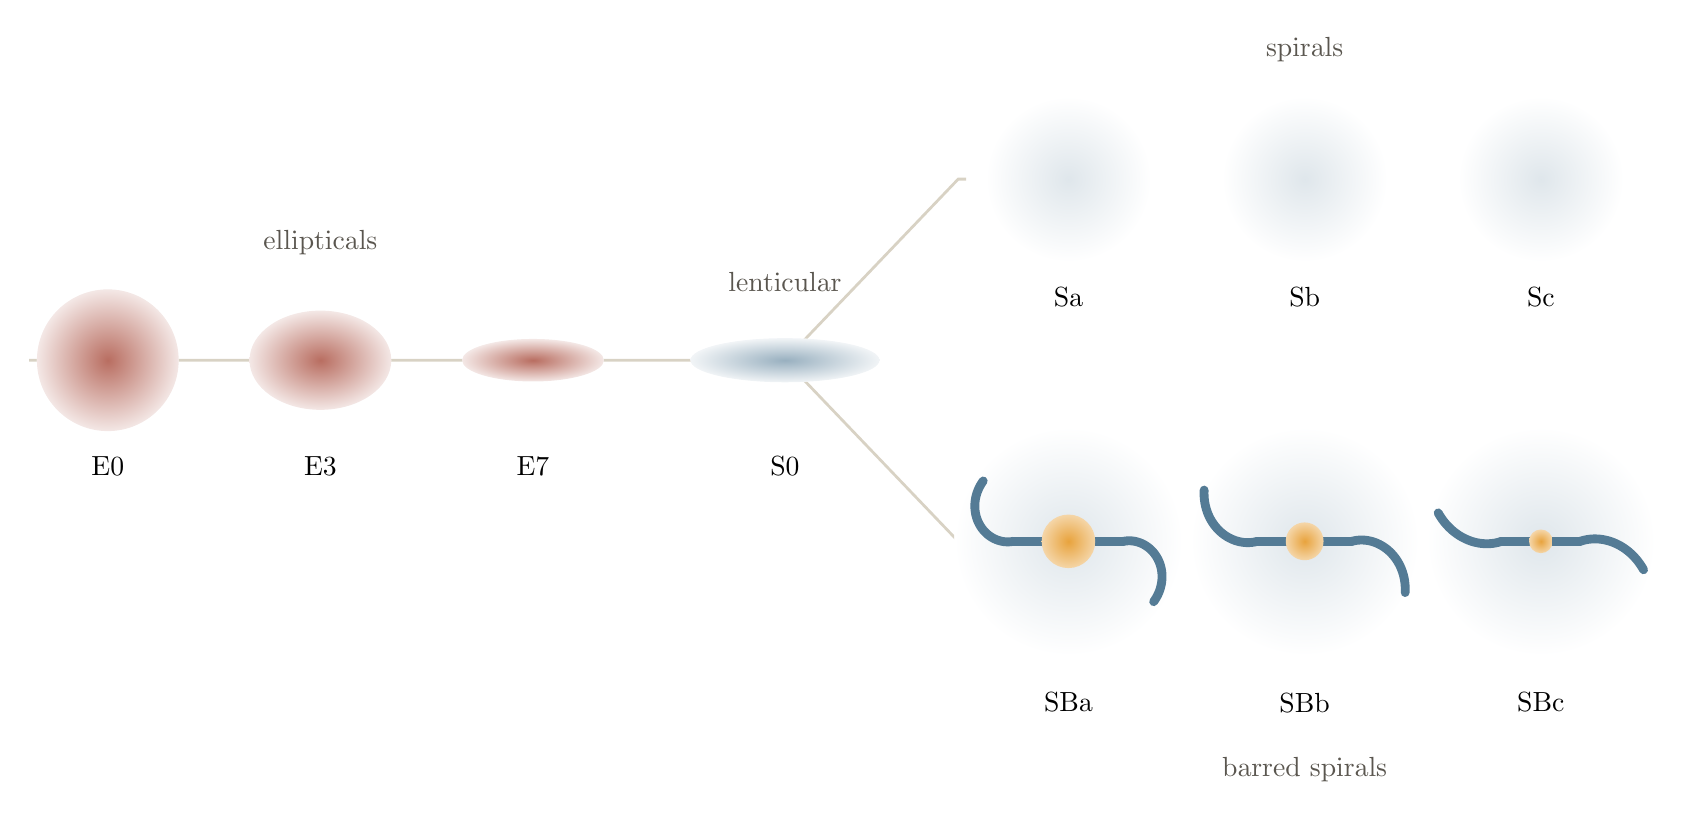
\begin{tikzpicture}[>={Stealth[length=2mm]}]
  % ---- fork lines
  \draw[linecol, line width=1pt] (-1,0) -- (8.6,0) -- (10.8,2.3) -- (10.9,2.3);
  \draw[linecol, line width=1pt] (8.6,0) -- (10.8,-2.3) -- (10.9,-2.3);
  % ---- ellipticals: E0, E3, E7 (flattening n/10)
  \foreach \x/\n in {0/0, 2.7/3, 5.4/7}{
    \begin{scope}[shift={(\x,0)}]
      \pgfmathsetmacro{\yr}{0.9*(1-\n/10)}
      \fill[white] (0,0) ellipse (0.9 and \yr);
      \shade[inner color=accent!75!white, outer color=accent!12!white] (0,0) ellipse (0.9 and \yr);
      \node[below=0.2cm] at (0,-0.9) {E\n};
    \end{scope}
  }
  % ---- lenticular S0, seen edge-on-ish: bulge plus smooth disk, no arms
  \begin{scope}[shift={(8.6,0)}]
    \fill[white] (0,0) ellipse (1.2 and 0.28);
    \shade[inner color=astroblue!45!white, outer color=astroblue!6!white] (0,0) ellipse (1.2 and 0.28);
    \bulge{0.45}{0.34}{0}
    \node[below=0.2cm] at (0,-0.9) {S0};
  \end{scope}
  % ---- ordinary spirals
  \foreach \x/\rb/\b/\nm in {12.2/0.40/0.13/Sa, 15.2/0.22/0.22/Sb, 18.2/0.12/0.36/Sc}{
    \begin{scope}[shift={(\x,2.3)}]
      \fill[white] (0,0) circle (1.05);
      \shade[inner color=astroblue!14!white, outer color=white] (0,0) circle (1.05);
      \arms{\rb}{\b}{1.0}{0}
      \bulge{\rb*1.1}{\rb*1.1}{0}
      \node[below=0.2cm] at (0,-1.05) {\nm};
    \end{scope}
  }
  % ---- barred spirals. Bar from -L to L. Arm 1 is a log spiral about a pole (L,-c) below the bar tip,
  % so it leaves the tip along the bar and then curls down. Arm 2 is arm 1 turned by 180 degrees.
  \foreach \x/\L/\c/\b/\sm/\g/\nm in {12.2/0.7/0.35/0.2/2.4/0.34/SBa, 15.2/0.6/0.42/0.28/1.9/0.24/SBb, 18.2/0.5/0.5/0.35/1.4/0.15/SBc}{
    \begin{scope}[shift={(\x,-2.3)}]
      \fill[white] (0,0) circle (1.45);
      \shade[inner color=astroblue!14!white, outer color=white] (0,0) circle (1.45);
      \foreach \rot in {0,180}{
        \draw[astroblue!75, line width=3.2pt, rotate=\rot, domain=0:\sm, samples=60, smooth, line cap=round]
          plot ({\L+\c*exp(\b*\x)*cos((pi/2-\x) r)}, {-\c+\c*exp(\b*\x)*sin((pi/2-\x) r)});
      }
      \draw[astroblue!75, line width=3.2pt, line cap=round] (-\L,0) -- (\L,0);
      \shade[inner color=sunyellow, outer color=sunyellow!45!white] (0,0) circle (\g);
      \node[below=0.2cm] at (0,-1.6) {\nm};
    \end{scope}
  }
  % ---- group labels
  \node[muted] at (2.7,1.5) {ellipticals};
  \node[muted] at (8.6,1.0) {lenticular};
  \node[muted] at (15.2,3.95) {spirals};
  \node[muted] at (15.2,-5.2) {barred spirals};
\end{tikzpicture}
\end{document}
